\documentclass{book} 

\usepackage{graphicx}
\usepackage{amsmath}
\usepackage{algorithm}
\usepackage{algpseudocode}
\usepackage{float}
\usepackage{hyperref}
\usepackage{placeins}

\usepackage{tikz}
\usetikzlibrary{arrows}
\usetikzlibrary{snakes}
\usetikzlibrary{decorations.pathmorphing}

\hypersetup{
	colorlinks,
	citecolor=black,
	filecolor=black,
	linkcolor=black,
	urlcolor=black
}

\title{Solutions of Introduction to Algorithms}
\author{Saman Saadi}
\date{} 

\begin{document}
	\frontmatter
	\maketitle
%	\newpage
	\tableofcontents
	\mainmatter
	\chapter{Dynamic Programming}
	\section{Rod cutting}	
	\paragraph{Exercise 2}
	No it cannot always produce an optimal solution. Consider the following example.
	\begin{table}[H]
		\centering
		\begin{tabular}{r||c|c|c}			
			$l_i$ & 1 & 2 & 3\\
			\hline
			$p_i$ & 1 & 50 & 72 \\
			\hline
			$\frac{p_i}{l_i}$ & 1 & 25 & 24
		\end{tabular}
	\end{table}
	For n = 3 the greedy approach cut the rod in 2 pieces. The length of one of them is 2 and the other's is 1. So the profit is $50\$ + 1\$ = 51\$$. But the optimal solution is to keep the rod intact so the profit is $72\$$.
	\paragraph{Exercise 3}
	We can keep the rod intact so we don't need to incur the fixed cost c or we can have at least one cut. We need to choose the best solution among all of them:
	\begin{equation*}
	r(i) = \begin{cases}
	\max\limits_{1 \leq k < n}(p_i, r(i - k) + p_k - c) & i > 0 \\
	0 & i = 0
	\end{cases}
	\end{equation*}
	So the solution is $r(n)$. We have n distinct subproblem. In each step we need to choose between keeping the rod intact or have at least one cut which divide the rod into two pieces. The length of one of them is k and the other's $n - k$. We don't know the exact value of k so we need to try all possible values. This can be done in $O(n)$. Therefore the overall running time is $O(n^2)$
	
	\begin{algorithm}
		\begin{algorithmic}[1]
			\Function{f}{p, n, c}
			\State let r[0..n] be a new array
			\State $r[0] \gets 0$
			\For{$\text{j from 1 to n}$}
			\State $q \gets p[j]$
			\For{i from 1 to $j - 1$}
			\State $q = max(q, r[j - i] + p[i] - c)$
			\EndFor
			\State r[j] = q
			\EndFor
			\State \Return $r[n]$
			\EndFunction
		\end{algorithmic}
	\end{algorithm}
	\section{Matrix-chain multiplication}
	\paragraph{Exercise 4}
	I've used the following equations:
	\begin{align}
	\sum_{i = 1}^{n} i &= \frac{n(n + 1)}{2}\\
	\sum_{i = 1}^{n} i^2 &= \frac{n(n + 1)(2n + 1)}{6}
	\end{align}
	Each node of the graph represents a distinct sub-problem. Suppose we have two nodes v and u. There is an edge from v to u, if the solution of subproblem v is depended on subproblem u. In other words, there is an edge from m[i, j] to all m[i, k] and m[k + 1, j] for $i \le k < j$. \\
	Usually $|V|$ determines space complexity and $|V| + |E|$ time complexity. we know for every subprobelm m[i, j], $j \ge i$. Hence we have $n - i + 1$ subproblems which starts with $A_i$. So the number of vertices is:
	\begin{equation}
	\begin{split}
	|V| &= \sum_{i = 1}^{n}{n - i + 1} \\
	&= \sum_{i=1}^{n}i \\
	&= \frac{n(n + 1)}{2}
	\end{split}
	\end{equation}
	Hence the space complexity is is $O(n^2)$. We don't use all of the array cells when $j < i$. So we waste $\frac{n^2 - n}{2}$ of allocated array. By analyzing lines 5 - 10 of MATRIX-CHAIN-ORDER pseudocode in the text book we can compute the number of edges.
	\begin{figure}[h!]
	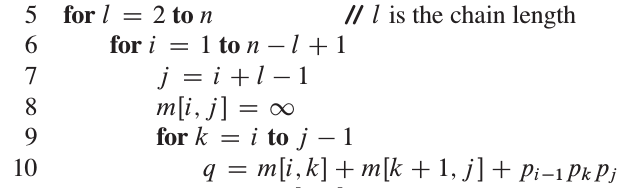
\includegraphics[width=\linewidth]{images/15/15-2-4.png}
	\end{figure}
	As you can see in line 10, m[i, j] is depends on two subproblem m[i, k] and m[k + 1, j]. We visit each distinct subproblem exactly once. So by counting the outdegree of each node we can calculate the number of edges in a directed graph:
	\begin{equation}
	\begin{split}
	|E| &= \sum_{l = 2}^{n}\sum_{i=1}^{n - l + 1}\sum_{k = i}^{i+l-2}2 \\
	&= \sum_{l=2}^{n}\sum_{i=1}^{n-l+1}2(l-1) \\
	&= 2\sum_{l=2}^{n}(n - l + 1)(l-1) \\
	&= 2\sum_{l=2}^{n}(n -(l - 1))(l-1) \\
	&= 2\sum_{l=1}^{n-1}(n-l)l \\
	&= 2(\sum_{l=1}^{n-1}nl - \sum_{l=1}^{n-1}l^2) \\
	&= 2(n\sum_{l=1}^{n-1}l - \sum_{l=1}^{n-1}l^2) \\
	&= 2[n\frac{(n - 1)n}{2} - \frac{(n - 1)(n)(2n - 1)}{6}] \\
	&= n^2(n - 1) - \frac{n(n-1)(2n-1)}{3} \\
	&= \frac{3n^2(n-1)-n(n-1)(2n-1)}{3} \\
	&= \frac{n(n-1)(3n-2n+1)}{3} \\
	&= \frac{n(n-1)(n+1)}{3}\\
	&= \frac{n(n^2-1)}{3}\\
	&= \frac{n^3 - n}{3}
	\end{split}
	\end{equation}
	So the running time is $|V| + |E| = \frac{n^2 + n}{2} + \frac{n^3 - n}{3} = O(n^3)$
	\section{Elements of dynamic programming}
	\paragraph{Exercise 2}
	Each node is filled with (p, r). p is the index of leftmost element and r is the index of rightmost element of array which the subprolem wants to sort. As you can see there is no overlapping between subproblems so dynamic programming is not a good idea for merge sort. In other words, we don't see a previously solved subproblem again and we only waste memory. As a general rule if the subproblem graph is a tree, dynamic programming cannot be applied.
	\begin{figure*}[h!]
		\centering
		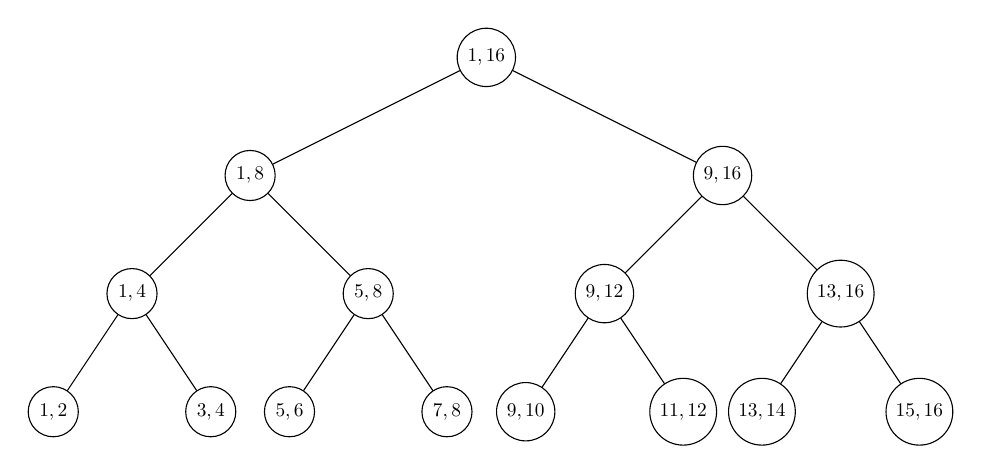
\begin{tikzpicture}[level/.style={sibling distance=60mm/#1}]
		\tikzset{vertex/.style = {shape=circle,draw,scale=0.7}}
			\node[vertex] (a){$1, 16$}
				child {node[vertex] (b) {$1, 8$}
						child {node[vertex] (d) {$1, 4$}
							child {node[vertex] (h) {$1, 2$}}
							child {node[vertex] (i) {$3, 4$}}
							}
						child {node[vertex] (e) {$5, 8$}
							child {node[vertex] (j){$5, 6$}}
							child {node[vertex] (k){$7, 8$}}
							}
					}
				child {node[vertex] (c) {$9, 16$}
					child {node[vertex] (f) {$9, 12$}
						child {node[vertex] (l){$9, 10$}}
						child {node[vertex] (m){$11, 12$}}
						}
					child {node[vertex] (g) {$13, 16$}
						child {node[vertex] (n){$13, 14$}}
						child {node[vertex] (o){$15, 16$}}
						}
					}
				;
		\end{tikzpicture}
	\end{figure*}
	\chapter{Amortized Analysis}
	\section{Aggregate analysis}
	\paragraph{Exercise 1}
	No it doesn't hold. The maximum number of pops, including multipop, is proportional to the number of previous push operations. If we can only push one item, the number of pushed elements is at most $n$. If we add a new operation named multipush, then the number of pushed items is at most $n \times k$. So the amortized cost is $O(k)$. For example we can have two operations. One is multipushing $10^9$ items and the other is multipopping $10^9$ items. It is obvious the total cost is not $O(n) = O(2)$ and is $O(nk) = O(2 \times 10^9)$.
	\paragraph{Exercise 2}
	The following pseudo-code explains how to implement DECREMENT.
	\begin{algorithm*}[h!]
		\begin{algorithmic}[1]
			\Function{DECREMENT}{A}
			\State $i = 0$
			\While{$i < A.length \text{ and } A[i] == 0$}
			\State $A[i] = 1$
			\State $i = i + 1$
			\EndWhile
			\If{$i < A.length$}
			\State $A[i] = 0$
			\EndIf
			\EndFunction
		\end{algorithmic}
	\end{algorithm*}
	The worst case happens when we start with 0 and then decrements it to get $2^k - 1$ which all bits are set to 1 and then increments it to get 0. We repeat this loop until we have n operations. For $n = 4$ and $k = 3$ we have:
	\begin{align*}
		&000 \\
		&111 \\
		&000 \\
		&111
	\end{align*}
	\section{Accountant method}
	For another example of "accountant method" see exercise 5 of \ref{sec:Representation of graphs}.
	\chapter{Elementary Graph Algorithms}
	\section{Representation of graphs}
	\label{sec:Representation of graphs}
	\paragraph{Exercise 1}
	We know that $adj[u]$ is a list. Depends on the list implementation, it can take $O(1)$ to determine its size. In that case the running time for finding the out-degree of each vertex is $O(V)$. If we cannot determine size of the list in $O(1)$, then the overall running time of algorithm is $O(V + E)$. \\
	The running time for finding in-degree of each vertex is $O(V + E)$.
	\paragraph{Exercise 3}
	For adjacency-matrix it takes $O(V^2)$ and for adjacency-list it takes $O(V + E)$.
	\begin{algorithm}[h!]
		\caption{$G'$ using adjacency matrix}
		\begin{algorithmic}[1]
			\Function{TransposeGraph}{G}
				\State Let $G'$ be a new graph
				\State $G' \gets G$
				\ForAll{$u \in V$}
					\ForAll{$v \in V$}
						\State $G'.A[v][u] = G.A[u][v]$
					\EndFor
				\EndFor
				\State \Return $G'$
			\EndFunction
		\end{algorithmic}
	\end{algorithm}
	\begin{algorithm*}[h!]
		\caption{$G'$ using adjacency list}
		\begin{algorithmic}[1]
			\Function{TransposeGraph}{G}
				\State Let $G'$ be a new graph
				\State $G'.V = G.V$
				\ForAll{$u \in G.V$}
					\ForAll{$v \in G.Adj[u]$}
						\State $G'.Adj[v].insert(u)$
					\EndFor
				\EndFor
			\EndFunction
		\end{algorithmic}
	\end{algorithm*}
	\FloatBarrier
	\paragraph{Exercise 4}
	We create a new adjacency-list for $G'$ called $adj$. For each vertex $u$ in $G$, suppose $v$ is its neighbor. If $u \ne v$, then $adj[u].insert(v)$ and $adj[v].insert(u)$. If there are multiple edges between $u$ and $v$, we see $v$ as $u$'s neighbor more than once. So if the last element if $adj[v]$ is $u$, it means there are more than one edges between them so we shouldn't insert $v$ again. Traversing $G$ takes $O(V + E)$. Finding out there are more than one edge between two vertices is $O(1)$. So the overall running time is $O(V + E)$. Note that I supposed $G$ is also undirected.
	\begin{algorithm}[h!]
		\begin{algorithmic}[1]
			\Function{f}{G}
			\State $\text{let }G' \text{ be a new graph}$
			\State $G'.V = G.V$
			\ForAll{$u \in G.V$}
				\ForAll{$v \in G.adj[u]$}
					\If{$u \ne v \land G'.adj[v].last() \ne u$}
						\State $G'.adj[v].insert(u)$		
					\EndIf
				\EndFor
			\EndFor
			\State \Return $G'$
			\EndFunction
		\end{algorithmic}
	\end{algorithm}
	\paragraph{Exercise 5}
	The running time of matrix-list implementation is $O(V^3)$. For analyzing the running time of adjacency-list implementation we can use amortized analysis. We use "accountant method".
	\begin{enumerate}
		\item[] $\boldsymbol{in_u:}$ The number of edges that enter $u$
		\item[] $\boldsymbol{out_u:}$ The number of edges that leave $u$
		\item[] $\boldsymbol{e_u:}$ And edge from u to an arbitrary vertex $v \ne u$
	\end{enumerate}
	We assign to all $e_u$ cost $c_{e_u} = 1 + in_u$. Because by traversing the graph, we visit $e_u$ at least once (line \ref{MakeSquareGraph:1-path}). For each edge that enters $u$ we visit or revisit $e_u$ (lines \ref{MakeSquareGraph:2-path:1} - \ref{MakeSquareGraph:2-path:2}). We know that $\sum_{u = 1}^{|V|}{in_u} + \sum_{u = 1}^{|V|}{out_u} = 2|E|$. So we can easily calculate the total cost.
	\begin{equation*}
		\begin{split}
		\sum_{e_u \in E}{c_{e_u}} &= \sum_{e_u \in E}{1 + in_u} \\
		&= \sum_{e_u \in E}{1} + \sum_{u = 1}^{|V|}{in_u} \\
		&= |E| + \sum_{u = 1}^{|V|}{in_u} \\
		&\le 3|E|
		\end{split}
	\end{equation*}
	We execute line \ref{MakeSquareGraph:1-path} at most $|E|$ times and lines \ref{MakeSquareGraph:2-path:1} - \ref{MakeSquareGraph:2-path:2} at most $2|E|$ times. So the total running time of algorithm using adjacency-list is $O(|V| + 3|E|) = O(V + E)$.
	\begin{algorithm*}[h!]
		\caption{Finding square graph using matrix-list}
		\begin{algorithmic}[1]
			\Function{MakeSquareGraph}{G}
				\State Let $G'$ be a new Graph
				\Comment $G.A[1..|V|, 1..|V|]$
				\ForAll{$u \in G.V$}
					\ForAll{$v \in G.V$}
						\State $G'.A[u][v] = G.A[u][v]$
						\Comment 1-edge paths
						\If{$G.A[u][v] = 1$}
							\ForAll{$k \in G.V$}
								\State $G'.A[u][k] = G.A[v][k]$
								\Comment 2-edge paths
							\EndFor
						\EndIf
					\EndFor
				\EndFor				
			\EndFunction
		\end{algorithmic}
	\end{algorithm*}
	\begin{algorithm*}[h!]
		\caption{Finding square graph using adjacency-list}
		\begin{algorithmic}[1]
			\Function{MakeSqureGraph}{G}
				\State Let $G'$	be a new graph
				\State $G'.V = G.V$
				\ForAll{$u \in G.V$}
					\ForAll{$v \in G.Adj[u]$}
						\State $G'.Adj[u].insert(v)$ \label{MakeSquareGraph:1-path}
						\Comment 1-edge paths
						\ForAll{$w \in G.Adj[v]$} \label{MakeSquareGraph:2-path:1}
							\State $G'.Adj[u].insert(w)$ \label{MakeSquareGraph:2-path:2}
							\Comment 2-edge paths
						\EndFor						
					\EndFor
				\EndFor
			\EndFunction
		\end{algorithmic}
	\end{algorithm*}
	\FloatBarrier
	\paragraph{Exercise 6}
	Suppose $A$ is an adjacency matrix for $G$.
	\begin{equation*}
		A[i, j] = \begin{cases}
		1 & \text{i cannot be a universal sink} \\
		0 & \text{j cannot be a universal sink}
		\end{cases}
	\end{equation*}
	The following algorithm find the universal sink in $O(V)$. In each step we remove one vertex from all candidates for "universal sink". It takes $O(V)$ to have only one candidate. To determine that candidate is indeed a universal sink we need $O(2V)$ operations. So the overall running time of algorithm is $O(V) + O(2V) = O(V)$.
	\begin{algorithm*}[h!]
		\begin{algorithmic}[1]
			\Function{getUniversalSink}{G}
				\State $A = G.A$
				\Comment $A[1..|V|, 1..|V|]$
				\State $u \gets 1$								
				\While{$u \le |V|$}
					\State $v \gets u + 1$
					\State $sink \gets u$
					\Comment Vertices from $sink$ to $|V|$ can be universal sink					
					\While{$v \le |V| \land A[u, v] = 0$}
						\State $v \gets v + 1$
						\Comment $v$ cannot be a universal sink
					\EndWhile
					\State $u \gets v$
					\Comment $u$ to $v - 1$ cannot be a universal sink
				\EndWhile
				\For{$c$ from $1$ to $sink - 1$}
					\If{$A[sink, c] \ne 0$}
						\State \Return "No universal sink"
					\EndIf
				\EndFor
				\For{$r \in V - \{sink\}$}
					\If{$A[r, sink] \ne 1$}
						\State \Return "No universal sink"
					\EndIf
				\EndFor
				\State \Return sink
			\EndFunction
		\end{algorithmic}
	\end{algorithm*}
	\FloatBarrier
	\paragraph{Exercise 7}
	We know that $B$ is an $V \times E$ matrix which we show it as $B_{V \times E}$. By definition $B^T$ is an $E \times V$ matrix which we show it as $B_{E \times V}^T$. We define $P_{V \times V} = B_{V \times E} \times B_{E \times V}^T$.
	\begin{equation*}
		p[i, j] = \sum_{k = 1}^{E}b[i, k] \times b^T[k, j]
	\end{equation*}
	We consider two cases.
	\begin{enumerate}
		\item $\boldsymbol{i \ne j:}$ It is impossible that both $b[i, k]$ and $b[k, j]$ have the value of "1". Because the k\textsuperscript{th} edge cannot enter both vertices $i$ and $j$. With the same argument we can prove that both of them cannot have value of "-1". If the k\textsuperscript{th} edge connect i to j, then $b[i, k] = -1$ and $b^T[k, j] = 1$. Otherwise both have value of zero. In other words, for $i \ne j$ the value of $p[i, j]$ is the number of edges between $i$ and $j$.
		\item $\boldsymbol{i = j:}$ It is obvious both $b[i, k]$ and $b[k, i]$ should have the same value. In this case $p[i, i]$ is the sum of all edges that enter and leave the vertex $i$.
	\end{enumerate}
	\begin{equation*}
		p[i, j] = \begin{cases}
		\text{number of edges between i and j} & i \ne j \\
		indegree(i) + outdegree(i) & i = j
		\end{cases}
	\end{equation*}
	\section{Breadth-first search}
	\paragraph{Exercise 8}
	It is easy to prove that the first and last vertex of the diameter is a leaf. Choose an arbitrary vertex $s$ and perform BFS on the graph. The vertex that has maximum number of edges from $s$ is one of the diameter's endpoints which we call it $u$. Then run another BFS from $u$ to get vertex $v$ which has maximum number of edges from $u$. This is the diameter.
	\paragraph{exercise 9}
	This undirected graph is equivalent to a directed graph which for all $u, v \in V$, $(u, v), (v, u) \in E$. We can use a modified version of DFS. Because we have both edges $(u, v)$ and $(v, u)$, we don't have "cross edges". We need to choose between "forward edges" or "back edges". In the following algorithm we use "forward edges" and skip "back edges".
	\begin{algorithm*}
		\begin{algorithmic}[1]
			\Function{DFS}{G, u}
				\State $u.color \gets Gray$
				\State $paths \gets \phi$
				\ForAll{$v \in G.Adj[u]$}
					\If{$v.color = White$} \Comment{Tree edge}
						\State $paths \gets \{(u, v)\} \cup DFS(G, v) \cup \{(v, u)\}$
					\ElsIf{$v.color = Black$} \Comment{Forward edge}
						\State $paths \gets paths \cup \{u, v\} \cup \{v, u\}$
					\EndIf
				\EndFor
				\State $u.color \gets Black$
				\State \Return paths
			\EndFunction
		\end{algorithmic}
	\end{algorithm*}
	\FloatBarrier
	\section{Depth-first search}
	\paragraph{Exercise 1}
	You can use the following facts. Suppose we have edge (u, v) and we consider loops as back edges.
	\begin{align*}	
	\begin{split}
		\text{\textbf{Tree edge: }} u.d &< v.d < v.f < u.f \\
		\text{\textbf{Forward edge: }} u.d &< v.d < v.f < u.f \\
		\text{\textbf{Back edge: }} v.d &\le u.d < u.f \le v.f \\
		\text{\textbf{Cross edge: }} v.d &< v.f < u.d < u.f \\
	\end{split}
	\end{align*}
	Note that when the graph is undirected we don't have "forward edge" and "cross edge". Because they are equivalent to "back edge" and "tree edge" respectively.
	\begin{table*}[h!]
		\centering
		\caption{Directed graph}
		\begin{tabular}{r|c|c|c}
			& white & gray & black \\
			\hline
			white & tree, back, forward, cross & back, cross & cross \\
			\hline
			gray & tree, forward  & tree, back, forward & tree, forward, cross \\
			\hline
			black & impossible & back & tree, back, forward, cross \\
		\end{tabular}
	\end{table*}
	\begin{table*}[h!]
		\centering
		\caption{Undirected graph}
		\begin{tabular}{r|c|c|c}
			& white & gray & black \\
			\hline
			white & tree, back & tree, back & impossible \\
			\hline
			gray & tree, back & tree, back & tree, back\\
			\hline
			black & impossible & tree, back & tree, back \\
		\end{tabular}
	\end{table*}
	\FloatBarrier
	\paragraph{Excercise 8}
	We need to show some examples which there is only one path from $u$ to $v$ and at least of one the edges in this path is not a tree edge. In the following examples the root of DFS trees is vertex $s$.
	\begin{figure*}[h!]
		\centering
		\caption{Counterexample using back edge}
		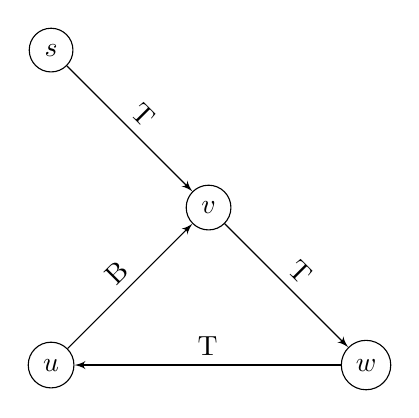
\begin{tikzpicture}		
			\tikzset{vertex/.style = {shape=circle,draw,minimum size=1.5em}}
			\tikzset{edge/.style = {->,> = latex'}}
			% vertices
			\node[vertex] (s) at (0, 0) {$s$};
			\node[vertex] (v) at (2, -2) {$v$};
			\node[vertex] (w) at (4, -4) {$w$};
			\node[vertex] (u) at (0, -4) {$u$};
			% edges
			\draw[edge] (s) -- (v) node[midway, above, rotate=-45] {T};
			\draw[edge] (v) -- (w) node[midway, above, rotate=-45] {T};
			\draw[edge] (w) -- (u) node[midway, above] {T};
			\draw[edge] (u) -- (v) node[midway, above, rotate=45] {B};
		\end{tikzpicture}
	\end{figure*}	
	\begin{figure*}[h!]
		\centering
		\caption{Counterexample using cross edge}
		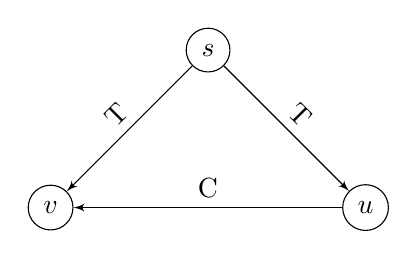
\begin{tikzpicture}
			\tikzset{vertex/.style = {shape=circle,draw,minimum size=1.5em}}
			\tikzset{edge/.style = {->,> = latex'}}
			% vertices
			\node[vertex] (s) at (0, 0) {$s$};
			\node[vertex] (u) at (2, -2) {$u$};
			\node[vertex] (v) at (-2, -2) {$v$};
			% edges
			\draw[edge] (s) -- (u) node[midway, above, rotate=-45] {T};
			\draw[edge] (u) -- (v) node[midway, above] {C};
			\draw[edge] (s) -- (v) node[midway, above, rotate=45] {T};
		\end{tikzpicture}
	\end{figure*}
	\FloatBarrier
	\paragraph{Excercise 9}
	Suppose we have edge (u, v) and we consider loops as back edges.
	\begin{align*}	
	\begin{split}
	\text{\textbf{Tree edge: }} u.d &< v.d < v.f < u.f \\
	\text{\textbf{Forward edge: }} u.d &< v.d < v.f < u.f \\
	\text{\textbf{Back edge: }} v.d &\le u.d < u.f \le v.f \\
	\text{\textbf{Cross edge: }} v.d &< v.f < u.d < u.f \\
	\end{split}
	\end{align*}
	As you can see only in cross edge the discovery of one endpoint is after the other finished. We need to prove that if there is a path from $u$ to $v$, it is possible to have $v.d > u.f$. In other words, edge $(v, u)$ is a cross edge and there is a path from $u$ to $v$ in which there is at least one edge which is not a tree edge. We can make counterexample even simpler by removing the cross edge. Note that the root of DFS tree is vertex $s$. In general if there is a cycle from $s$ to $u$ and $u$ to $s$, then it is possible $v.d > u.f$.
	
	\begin{figure*}[h!]
		\centering
		\caption{Counterexample using cross edge}
		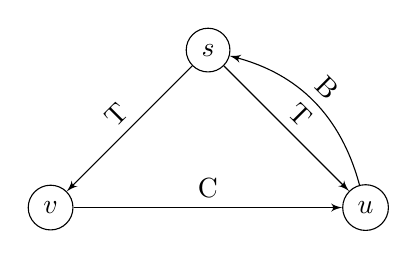
\begin{tikzpicture}
			\tikzset{vertex/.style = {shape=circle,draw,minimum size=1.5em}}
			\tikzset{edge/.style = {->,> = latex'}}
			% vertices
			\node[vertex] (s) at (0, 0) {$s$};
			\node[vertex] (u) at (2, -2) {$u$};
			\node[vertex] (v) at (-2, -2) {$v$};
			% edges
			\draw[edge] (s) -- (u) node[midway, above, rotate=-45] {T};
			\draw[edge] (v) -- (u) node[midway, above] {C};
			\draw[edge] (s) -- (v) node[midway, above, rotate=45] {T};
			\draw[edge] (u) edge[bend right] node [midway, above, rotate=-45] {B} (s);
		\end{tikzpicture}		
	\end{figure*}
	\begin{figure*}[h!]
		\centering
		\caption{Counterexample without cross edge}
		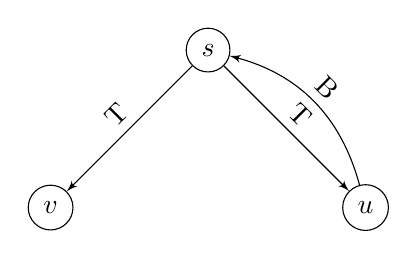
\begin{tikzpicture}
		\tikzset{vertex/.style = {shape=circle,draw,minimum size=1.5em}}
		\tikzset{edge/.style = {->,> = latex'}}
		% vertices
		\node[vertex] (s) at (0, 0) {$s$};
		\node[vertex] (u) at (2, -2) {$u$};
		\node[vertex] (v) at (-2, -2) {$v$};
		% edges
		\draw[edge] (s) -- (u) node[midway, above, rotate=-45] {T};
		\draw[edge] (s) -- (v) node[midway, above, rotate=45] {T};
		\draw[edge] (u) edge[bend right] node [midway, above, rotate=-45] {B} (s);				
		\end{tikzpicture}		
	\end{figure*}
	\begin{figure*}[h!]
		\centering
		\caption{General counterexample}
		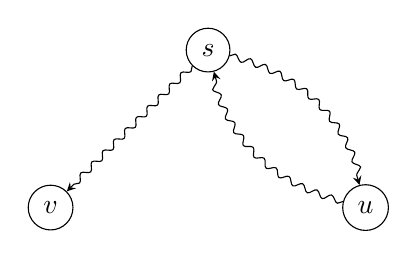
\begin{tikzpicture}
		\tikzset{vertex/.style = {shape=circle,draw,minimum size=1.5em}}
		\tikzset{edge/.style = {->,> = latex'}}
		\tikzset{snake it/.style={-stealth,
				decoration={snake, 
					amplitude = .4mm,
					segment length = 2mm,
					post length=0.9mm},decorate}}			
		% vertices
		\node[vertex] (s) at (0, 0) {$s$};
		\node[vertex] (u) at (2, -2) {$u$};
		\node[vertex] (v) at (-2, -2) {$v$};
		% edges
		\path[edge] (s) edge[bend left, snake it] (u);
		\path[edge] (s) edge[snake it] (v);
		\path[edge] (u) edge[bend left, snake it](s);				
		\end{tikzpicture}		
	\end{figure*}		
	\FloatBarrier
	
\end{document}
